\documentclass{beamer}
\usetheme{default}
\usepackage{graphicx}
\title{Trabajo Práctico:
	Cinemática de Robots}
\author{Equipo Droideka}


\begin{document}
\begin{frame}[plain]
    \maketitle
\end{frame}
\begin{frame}
    \frametitle{Frame Title}
\end{frame}

\begin{frame}[plain]
	\maketitle
\end{frame}



\begin{frame}
	\frametitle{Idea general}
	Sampling 3D del jacobiano, autovalor en heatmap y dirección del autovector como vector.
\end{frame}


% TODO: \usepackage{graphicx} required
\begin{figure}[h!]
	\centering
	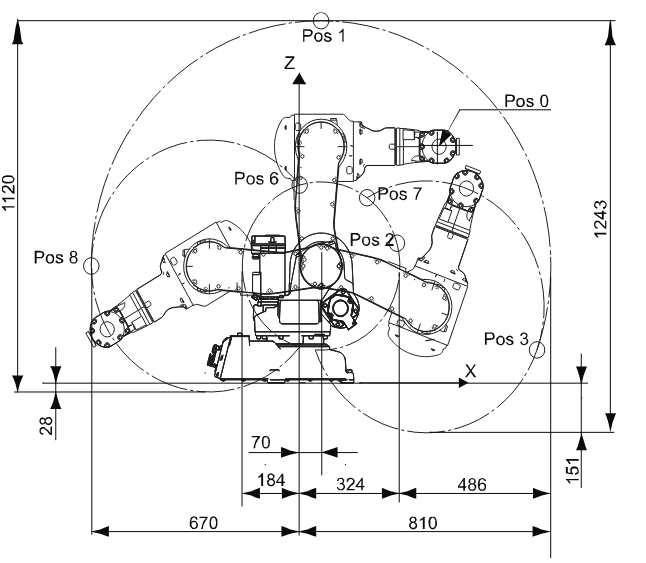
\includegraphics[width=0.7\linewidth]{imgs/screenshot001}
	\label{fig:screenshot001}
\end{figure}




\end{document}



